\documentclass[a4paper,oneside,12pt,DIV=12,titlepage]{scrartcl}

%Typography
\usepackage{fontspec}
\setromanfont{STIX Two Text}
\setsansfont{PT Sans}
\setmonofont{PT Mono}

\usepackage{microtype}

%Localization
\usepackage{polyglossia}
\setdefaultlanguage{ukrainian}
\PolyglossiaSetup{ukrainian}{indentfirst=true}

%Math typesetting
\usepackage{amsmath}
\usepackage{unicode-math}
\setmathfont{STIX Two Math}

\usepackage[retainorgcmds]{IEEEtrantools}

%Table typesetting
\usepackage{booktabs}

%Including graphics
\usepackage{graphicx}

\usepackage{subcaption} % side-by-side figures

%Drawing electrical circuits
%\usepackage{circuitikz}

%SI Units
\usepackage[]{siunitx}
\sisetup{output-decimal-marker = {,}} % Use comma as a decimal separator

%Itemize separator
\def\labelitemi{—}

%Definition of const
\newcommand\const{\text{const}}

%Definition of schematic element
\newcommand\schel[1]{\textit{#1}}

\begin{document}
	\begin{titlepage}
		\begin{center}
			Міністерство освіти і науки України\\
			Національний авіаційний університет\\
			Навчально-науковий Інститут\\
			Комп'ютерних інформаційних технологій\\
			Кафедра комп'ютеризованих систем управління
			
			\vspace{\fill}
				Лабораторна робота №2\\
				з дисципліни «Комп'ютерна електроніка»\\
				на тему: «Дослідження біполярного транзистора»\\
				Варіант №
				
			\vspace{\fill}
			
			\begin{flushright}
				Виконав:\\
				студент ННІКІТ СП-225\\
				Клокун Владислав\\
				Перевірив:\\
				Андрєєв О.В.
			\end{flushright}
			Київ 2017
		\end{center}
	\end{titlepage}
	
	\section{Мета та основні завдання роботи}
		\begin{enumerate}
			\item Ознайомитись з принципом дії, схемами ввімкнення і ВАХ біполярного транзистора.
			\item Набути практичних навичок у побудові вольт-амперних характеристик біполярного тразистора.
			\item Набути практичних навичок у побудові навантажувальної прямої транзистора і визначенні h-параметрів.
			\item Дослідити вплив положення робочої точки транзистора на форму вихідного сигналу.
			\item Вивчити схеми ввімкнення біполярних транзисторів і їхні вольт-амперні характеристики.
			\item Вивчити методику побудови навантажувальної прямої, вибору робочої точки і визначення h-параметрів.
			\item Освоїти методику побудови за вхідною напругою інших струмів і напруг біполярного транзистора.
		\end{enumerate}
		
	\section{Хід роботи}
		\begin{figure}[h]
			\centering
			\includegraphics[width=0.95\textwidth]{schematic-01.jpg}
			\caption{Принципова електрична схема віртуальної лабораторної установки}
		\end{figure}
		
		\subsection{Дослідження біполярного транзистора в статичному режимі}
			\subsubsection{Побудова вхідних вольт-амперних характеристик}
				Готуємо лабораторну установку до роботи. Для цього встановлюємо перемикачі \schel{SA1}, \schel{SA2}, \schel{SA3}, \schel{SA4} у положення «1», «2», «1», «2» відповідно. Вмикаємо осцилограф та встановлюємо такі налаштування:
				\begin{table}[!h]
				\centering
					\begin{tabular}{lll}
						Time Base & 0,2 ms/div & A/B, Auto\\
						Channel A & 2~mV/div & DC\\
						Channel B & 100 mV/div & DC\\
					\end{tabular}
				\end{table}
						
				Встановлюємо напругу $E_{\textnormal{К}} = \SI{0}{\volt}$ за допомогою потенціометра R7 (100\%). Вмикаємо лабораторну установку на моделювання. Змінюємо значення вхідної напруги $U_{\textnormal{БЕ}}$ за допомогою потенціометра \schel{R2} від 0 до 100\%. При цьому на екрані осцилографа з'явилась вхідна характеристика транзистора, знята при напрузі $U_{\textnormal{К}}$. Вимикаємо установку. Відкриваємо аналізатор графіків та встановлюємо такі налаштування:
				
				\begin{table}[!h]
					\centering
					\begin{tabular}{lllll}
						\multicolumn{5}{c}{\textbf{Left Axis}}\\
						Range & Minimum & 0 & Maximum & 0,01\\
						\multicolumn{5}{c}{\textbf{Bottom Axis}}\\
						Range & Minimum & 0 & Maximum & 0,01\\
						Divisions & Number & 0 & Precision & 1\\
					\end{tabular}
				\end{table}
						
				Перерисовуємо вхідну характеристику $U_{\textnormal{К}} = f(I_{\textnormal{Б}}), U_{\textnormal{К}} = \const$. Встановлюємо напругу $E_{\textnormal{К}} = \SI{10}{\volt}$ за допомогою потенціометра \schel{R7} (приблизно 70\%). Будуємо графік. Встановлюємо напругу $E_{\textnormal{К}} = \SI{20}{\volt}$ за допомогою потенціометра \schel{R7} (43\%). Будуємо графік.
				
				\begin{figure}[!h]
					\centering
					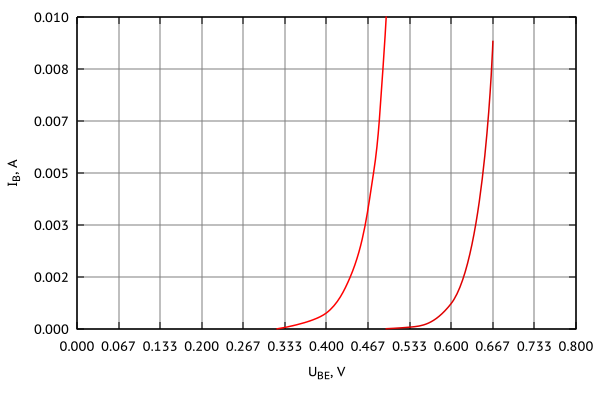
\includegraphics[width=0.7\textwidth]{plots/input-graphs-combined.pdf}
					\caption{Вхідна характеристика біполярного транзистора}
				\end{figure}
			
			\subsubsection{Побудова вихідних вольт-амперних характеристик}
				Готуємо лабораторну установку до продовження роботи. Для цього переводимо перемикач \schel{SA2} в положення «1». Змінюємо масштаби на осцилографі на такі значення:
				\begin{table}[!h]
				\centering
					\begin{tabular}{lll}
						Channel A & 200~mV/div & DC \\
						Channel B & 5~V/div & DC \\
					\end{tabular}
				\end{table}
				
				Встановлюємо колекторну напругу $U_{\textnormal{К}} = 0$ за допомогою потенціометра \schel{R7} зі значенням 100\%. Вмикаємо лабораторну установку на моделювання. Встановлюємо струм бази $I_{\textnormal{Б}} = \SI{632,5}{\micro\ampere}$ потенціометром \schel{R2} зі значенням приблизно 20\%. Змінюємо значення $U_{\textnormal{К}}$ від 0 до 40~В за допомогою потенціометра \schel{R7} зі значеннями від 100\% до 0\%. Вимикаємо лабораторну установку.
				
				Відкриваємо аналізатор графіків і встановлюємо такі налаштування:
				\begin{center}
					\begin{tabular}{lllll}
						\multicolumn{5}{c}{\textbf{Left Axis}}\\
						Range & Minimum & 0 & Maximum & 0,09\\
						\multicolumn{5}{c}{\textbf{Bottom Axis}}\\
						Range & Minimum & 0 & Maximum & 40\\
						Divisions & Number & 8 & Precision & 0\\
					\end{tabular}
				\end{center}
				
				Встановлюємо струм бази $I_{\textnormal{Б}} = \SI{2,23}{\milli\ampere}$ за допомогою потенціометра \schel{R2} зі значенням 30\%. Зарисовуємо другу характеристику.
				
				Встановлюємо струм бази $I_{\textnormal{Б}} = \SI{5,13}{\milli\ampere}$ за допомогою потенціометра \schel{R2} зі значенням 50\%. Зарисовуємо третю характеристику.
				
				Вимикаємо моделювання лабораторної установки та аналізатор графіків.
			
		\subsection{Дослідження біполярного транзистора в режимі посилення}
			Встановлюємо перемикач \schel{SA3} в положення «2». Встановлюємо напругу $E_{\textnormal{К}} = \SI{10}{\volt}$ за допомогою потенціометра \schel{R7} зі значенням 71\%. Задаємо вхідні напруги $U_{\textnormal{БЕ}} = \SI{392}{\milli\volt}$ і $I_{\textnormal{Б}} \approx \SI{0,65}{\micro\ampere}$ за допомогою потенціометра \schel{R2} зі значенням 15\%.
			
			Вимірюємо координати робочої точки на вихідній характеристиці за допомогою приладів \schel{PV2}, \schel{PA2}:
			\begin{IEEEeqnarray}{rCcCl}
				\schel{PV2} & = & U_{\textnormal{К1}} & = & \SI{10}{\volt}\\
				\schel{PA2} & = & I_{\textnormal{К}} & = &\SI{11}{\micro\ampere}
			\end{IEEEeqnarray}
			
			Таким чином, точка $A$ має координати $(\num{10}; \num{0,00011})$. Звертаємо увагу, що $\schel{PV3} = \schel{PV2}$.
			
			Збільшуємо вхідну напругу до $U_{\textnormal{БЕ}} \approx \SI{632}{\milli\volt}$ та напругу $I_{\textnormal{Б}} \approx \SI{3,15}{\milli\ampere}$ за допомогою потенціометра \schel{R2} зі значенням 44\%. 
			
			Вимірюємо координати другої робочої точки $I_{\textnormal{К2}}$, $U_{\textnormal{КЕ2}}$ за допомогою приладів \schel{PV2}, \schel{PA2}:
			\begin{IEEEeqnarray}{rCcCl}
				\schel{PV2} &=& U_{\textnormal{К2}} &=& \SI{3,778}{\volt}\\
				\schel{PA2} &=& I_{\textnormal{К2}} &=& \SI{52,39}{\milli\ampere}
			\end{IEEEeqnarray}
			
			Таким чином, точка $B$ має координати $\left(\num{3,778}; \num{0,05239}\right)$. Вимикаємо моделювання.
			
			За координатами двох точок на графіку сім'ї вихідних зарактеристик будуємо навантажувальну пряму (рис. \ref{fig:outputloadline}). Обчислюємо за законом Ома величину $R_{\textnormal{К}}$:
			\[
				R_{\textnormal{К}} = \frac{U_{\textnormal{КЕ}}}{I_{\textnormal{К}}} \approx \frac{\SI{7}{\volt}}{\SI{0,025}{\ampere}} \approx \SI{280}{\ohm}
			\]
			
			\begin{figure}[h]
				\centering
				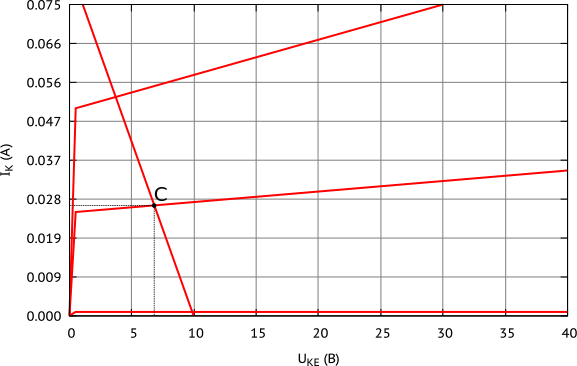
\includegraphics[width=0.7\textwidth]{plots/output-families-loadline-corrected.pdf}
				\caption{Сімейство вихідних характеристик з навантажувальною прямою}\label{fig:outputloadline}
			\end{figure}
			
		\subsection{Дослідження біполярного транзистора в режимі посилення гармонійних коливань}
			Досліджуємо біполярний транзистор у режимі посилення гармонійних коливань. Для цього на вході транзистора задаємо робочу точку по середині лінійної ділянки вхідних характеристик для $E_{\textnormal{К}} \approx 10$~В.
			
			Відкриваємо осцилограф і налаштовуємо його таким чином:
			\begin{center}
				\begin{tabular}{lll}
				Time Base & 0,5 ms/div & Y/T, Auto\\
				Channel A & 50~mV/div & AC\\
				Channel B & 200~mV/div & AC\\
				\end{tabular}
			\end{center}
			
			Відкриваємо вікно налаштувань генератора синусоїдних коливань і встановлюємо значення амплітуди вхідного струму $U_{\textnormal{ВХ}} = \SI{13}{\milli\volt}$ та частоту коливань $F = \SI{1}{\kilo\hertz}$. Підключаємо генератор до вхідного ланцюга біполярного транзистора, встановивши перемикач \schel{SA4} у положення «1», та вмикаємо генератор.
			
			Перерисовуємо осцилограми вхідної і вихідної напруг. Визначаємо амплітуди вхідної та вихідної напруг: $U_{\textnormal{Б}} = \SI{18,74}{\milli\volt}$, $U_{\textnormal{К}} = \SI{351,27}{\milli\volt}$.
			
			\begin{figure}[h]
				\centering
				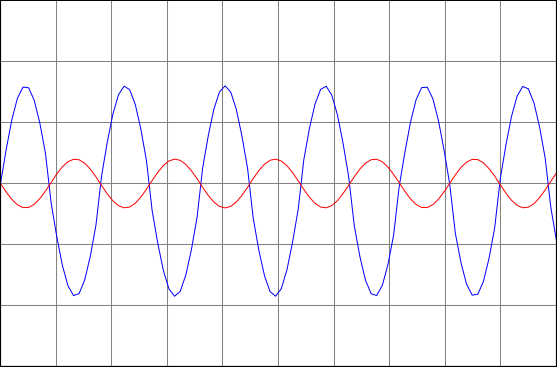
\includegraphics[width=0.6\textwidth]{plots/sine-waves-01-v02.pdf}
				\caption{Осцилограма вхідного та вихідного сигналів}
			\end{figure}
			
			За допомогою потенціометра \schel{R2} (71\%) зміщуємо робочу точку в область режиму насичення: $I_{\textnormal{Б}} \approx \SI{6,6}{\milli\ampere}$, $U_{\textnormal{БЕ}} \approx 647$~мВ. Перерисовуємо осцилограми вхідної і вихідної напруг. Визначаємо амплітуди вхідної та вихідної напруг: $U_{\textnormal{Б}} \approx \SI{17,35}{\milli\volt}$, $U_{\textnormal{К}} \approx \SI{325,43}{\milli\volt}$. Вимикаємо осцилограф і моделювання.
			
			\begin{figure}[h]
				\centering
				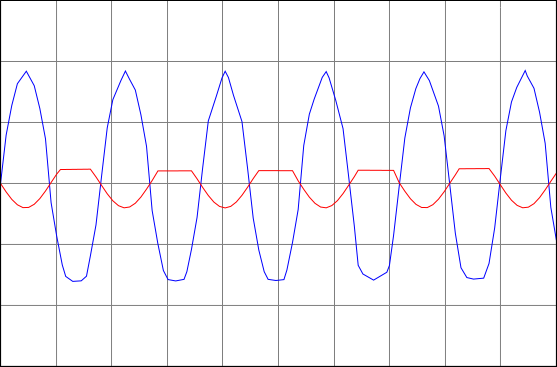
\includegraphics[width=0.6\textwidth]{plots/sine-waves-02-v01.pdf}
				\caption{Осцилограма вхідного та вихідного сигналів}
			\end{figure}
			
			Зазначимо, що зі зміною положення робочої точки змінилась амплітуда сигналів, а також стали помітними візуальні спотворення на осцилограмах.
			
	\section{Висновки}
		Виконавши лабораторну роботу №2 на тему «Дослідження біполярного транзистора» ми досягли таких цілей:
			\begin{enumerate}
				\item Ознайомились з принципом дії, схемами ввімкнення і вольт-амперними характеристиками біполярного транзистора.
				\item Набули практичних навичок з побудови вольт-амперних характеристик.
				\item Набули практичних навичок з побудови навантажувальної прямої транзистора.
				\item Дослідили вплив положення робочої точки транзистора на форму вихідного сигналу.
				\item Вивчили схеми ввімкнення біполярних транзисторів і їх вольт-амперні характеристики. 
				\item Освоїли методику побудови за вхідною напругою інших струмів і напруг біполярного транзистора.
			\end{enumerate}
			
		%Виконавши дослідження роботи біполярного транзистора у статичному режимі, ми переконались, що при напрузі $U_{\textnormal{КЕ}} = 0$ вхідна вольт-амперна характеристика дійсно починається на початку координат. Крім того, ми удостовірились, що при збільшенні $U_{\textnormal{КЕ}}$ ($U_{\textnormal{КЕ}} > 0$) вхідна вольт-амперна характеристика зміщується вправо та вниз.
		
		Виявлено, що при збільшенні $U_{\textnormal{КЕ}}$ ($U_{\textnormal{КЕ}} > 0$) вхідна вольт-амперна характеристика зміщується вправо та вниз. Крім того, сигнал, що проходить через біполярний транзистор у режимі посилення гармонійних коливань, піддається нелінійним спотворенням.
		
\end{document}